\normalfalse \difficiletrue \tdifficilefalse
\correctionfalse

%\UPSTIidClasse{11} % 11 sup, 12 spé
%\newcommand{\UPSTIidClasse}{12}

\exer{Système bielle manivelle  $\star\star$ \label{CIN:01:B2:12:12}}
\setcounter{question}{0}\marginnote{\xpComp{CIN}{01}}%\UPSTIcompetence{B2-12}
\index{Compétence B2-12}\index{Compétence CIN-01}
\index{Bielle Manivelle}
\index{Moteur}
\ifcorrection
\else
\marginnote{\textbf{Pas de corrigé pour cet exercice.}}
\fi

\ifprof
\else
Soit le mécanisme suivant. On a $\vect{AB}=R\vect{i_1}$ et $\vect{CB}=L\vect{i_2}$. De plus, 
$R=\SI{10}{mm}$ et $L=\SI{20}{mm}$. 

\begin{marginfigure}
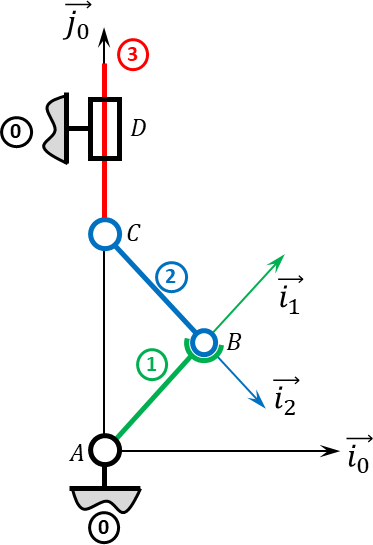
\includegraphics[width=\linewidth]{12_01}
\end{marginfigure}
\fi

\question{Tracer le graphe des liaisons.}
\ifprof
\else
\fi

\question{Retracer le schéma cinématique pour $\theta(t)=\dfrac{\pi}{2}\,\text{rad}$.}
\ifprof
\else
\fi

\question{Retracer le schéma cinématique pour $\theta(t)=-\dfrac{\pi}{2}\,\text{rad}$.}
\ifprof
\else
\fi


\question{En déduire la course de la pièce \textbf{3}.}
\ifprof
\else
\fi



\ifprof
\else
\marginnote{Corrigé  voir \ref{CIN:01:B2:12:12}.}
\fi